\chapter{Diseño del experimento}

Utilizando estudios previos de ambas variantes del español pudimos obtener las reglas definidas en el capítulo anterior. Recordemos que estas describen la diferencia entre cada uno de los dos grupos. Vamos a proponer realizar un experimento para poder extraer la información fonética de los mismos. La idea será realizar una serie de actividades donde el hablante sea grabado y esas actividades hagan hincapié en estas diferencias descriptas. A continuación vamos a describir el experimento en más detalle.

\section{Elección de las frases}

El acento se potencia cuando se realiza habla espontánea. Utilizando este concepto intentaremos que el hablante lo diga de forma lo más natural posible. Es por ello que se nos ocurrió como actividad pronunciar frases popularmente conocidas. Si el hablante conoce la frase y la utiliza con frecuencia entonces es más fácil que su pronunciación sea utilizando habla espontánea. Con esta idea vamos a cubrir las reglas 2 a 6.

También tenemos que hacer hincapié en las sílabas acentuadas. Recordemos que en el capítulo anterior la regla 1 nos decía que había una diferencia en la duración de la silaba previa a la acentuada. Esta sílaba varía según que tipo de palabra es la acentuada. No es lo mismo utilizar una palabra aguda o esdrújula. Para cubrir estar reglas utilizamos un esquema de frases con una estructura fija pero que varía sus palabras. Este esquema se llama AMPER.

A continuación veremos cada grupo en más detalle. 

\paragraph{Descripción de los 2 tipos de frases}
%-Descripción de los 2 grupos. Porque cada uno. Espontaneidad vs Regla 1

Vamos a tener dos formas de grabaciones: 

\begin{itemize}
  \item Frases comunes que tratan de cubrir la espontaneidad. Estas frases van a cubrir las reglas 2 a 6. Estas tienen que ver con la duración y la pronunciación de distintos fonémas.  
  \item Frases AMPER que tratan de cubrir el acento barriendo por cada tipo de acentuación. Estas corresponden a la regla 1 que hace incapié en la longitud de la sílaba anterior a la acentuada.
\end{itemize}

A continuación vemos las reglas en sus dos conjuntos.

\subsection{Frases utilizadas}

\begin{figure}[h!]
    \centerline{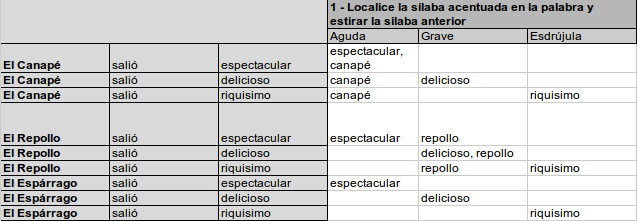
\includegraphics[width=1\textwidth]{reglas_AMPER} }
    \caption{Frases AMPER}
    \label{fig21}
\end{figure}

\begin{figure}[h!]
    \centerline{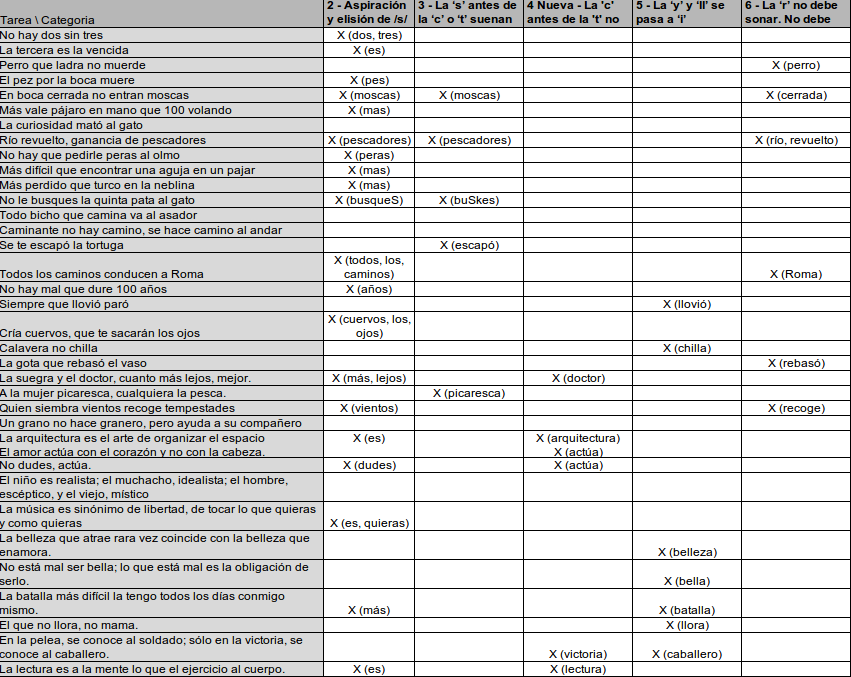
\includegraphics[width=1\textwidth]{frases_inf} }
    \caption{Frases conocidas}
    \label{fig22}
\end{figure}

\subsection{Utilizar frases conocidas}

Como afirmamos antes, se utilizaron frases comunes para poder obtener los acentos de cada grupo de forma natural. Se pensó que si se graba una frase popular, el hablante al estar acostumbrado a decirla no iba a poder evitar impregnarle el su acento. Todas las frases conocidas utilizadas se pueden ver en la Figura \ref{fig22}.

Algo interesante es que una misma frase puede extraer atributos para varias reglas. Por ejemplo: la frase \textit{En la pelea se conoce al soldado, sólo en la victoria se conoce al caballero} extrae atributos para las reglas 4 y 5. La palabra \textit{victoria} posee atributo para la regla 4 que nos propone medir la duración de la \textit{c} antes de la \textit{t}. Sucede igual con la palabra \textit{caballero} para la regla 5. Esta nos dice medir la duración de la \textit{ll}. De esta forma cada frase extrae los atributos lo mas posible. En la Figura \ref{fig22} podemos ver el desbalance entr la cantidad de frases utilizadas con respecto a sus reglas aplicadas. Más adelante veremos como impacta esto en las frases que vamos a pedir para grabar.

\subsection{Utilizar frases con esquema AMPER}

%AMPER-ARGENTINA: VARIABILIDAD RÍTMICA EN DOS CORPUS 
%Jorge A. Gurlekian LIS - Conicet y UBA jag@fmed.uba.ar 
%Reina Yanagida LIS y Universidad Municipal de Estudios Extranjeros de Kobe, Japón reinay@hotmail.co.jp 
%Mónica Noemí Trípodi LIS – UBA monica906@hotmail.com 
%Guillermo Toledo Conicet y Universidad Laval, Canadá guillermo.toledo@sympatico.ca 

Utilizamos este esquema para analizar todas las variantes posibles de la Regla 1. Recordemos que esa regla nos dice que hay que estirar la sílaba anterior a la acentuada. Esta regla es la más conocida y puede aparecer de varias formas. Es por eso que este esquema nos va a resultar muy útil. Para tomar este esquema nos basamos en el trabajo de \cite{amper}

Para el esquema AMPER se fija un patrón de estructura de frases y se va cambiando las palabras que utiliza. 
El esquema AMPER utilizado es: 
\begin{center}
\textit{Objeto+” salió “+Adjetivo} 
\end{center}
donde Objeto puede ser \textit{Canapé. Repollo, Espárrago}. Adjetivo puede ser \textit{espectacular, delicioso, riquísimo}. Utilizamos estas palabras ya que cubren por la acentuación de cada tipo de palabra, o sea pasa por agudas grave y esdrújula. 

Por ejemplo: \textit{El canapé salio delicioso}. Canapé tiene acento en la última sílaba. Es una palabra aguda. Mientras que delicioso es grave. En este ejemplo podemos analizar la sílaba anterior a la acentuada de estos dos grupos. Es importante armar la mayoría de las combinaciones para obtener muchas variantes de donde se encuentra el acento. De esta forma poder obtener muchísimas variantes con respecto a la Regla 1, que nos decía estirar la sílaba anterior a la acentuada. Todas las combinaciones se pueden ver en la Figura \ref{fig21}.

%También se agregó “El rábano salió horrible” que posee un acento en la primer sílaba.

\paragraph{Intercalando los dos tipos:}
Intercalaremos las frases comunes con las frases de AMPER para obtener las trazas de frases a grabar. Vamos a agregar 4 o 5 frases comunes, luego agregar 1 o 2 frases del esquema de AMPER y así sucesivamente hasta completar todas. La idea es no cansar al hablante con frases repetitivas y evitar que sepa de antemano que frase va a tener que grabar.

\paragraph{Siempre cada 5 grabaciones:}
La mínima cantidad de grabaciones que puede realizar un hablante son 5 grabaciones. Luego se le pregunta si quiere continuar grabando. Si acepta, se le agregan otras 5 grabaciones así sucesivamente hasta llegar a las 40 que es el total de grabaciones.

\section{Generación de trazas}

%Debemos definir qué frases y en que órden se debe decir durante el experimento. Este orden va a tener la condición de que en cada nueva frase agregada vamos a querer cubrir lo mayor posible el porcentaje de cubrimiento de cada una de las reglas. Utilizaremos un algoritmo goloso para generar la traza hasta poder cubrir el 100\% de cada regla.

%La idea del algoritmo para generar trazas se va a basar en utilizar la frase que mayor información aporte en cada paso. No es lo mismo grabar una frase que solo aporta información a la regla 2 que una que aporta a la regla 2, 3, 4. Por ello, en cada paso se va agregando una frase que no fue utilizada y además que aporte la mayor cantidad de información. Es importante aplicar esta idea ya que no sabemos cuanto tiempo va a querer/tener un hablante para realizar el experimento. Utilizando nuestro algoritmo, podemos afirmar que ya con 10 frases grabadas se cubre con todas las reglas propuestas anteriormente. En el gráfico podemos ver el desempeño de nuetro algoritmo. 

Definimos como va a ser el esquema general de las trazas, ahora debemos definir qué frases y en que orden se debe decir durante el experimento. Sucede que el orden que utilicemos va a ser crucial para tener muestras. No es lo mismo empezar por una frase que sólo referencia a una regla que a varias. Si referencia a varias reglas a la vez, en un sólo audio podremos sacarle más información.

Una traza es una lista de las frases que puede grabar un hablante. Un hablante al empezar se le dará una de estas y grabará sucesivamente en ese orden. Elegimos tener precalculada las trazas para evitar cálculos innecesarios a la hora de empezar el experimento. Es por eso que guardamos 10.000 trazas generadas. Entonces al ingresar un hablante nuevo al experimento se le dará una de estas trazas para que grabe.

La generación de trazas sigue el siguiente algoritmo:

\lstset{ %
language=C++,                % choose the language of the code
basicstyle=\footnotesize,       % the size of the fonts that are used for the code
numbers=left,                   % where to put the line-numbers
numberstyle=\footnotesize,      % the size of the fonts that are used for the line-numbers
stepnumber=1,                   % the step between two line-numbers. If it is 1 each line will be numbered
numbersep=5pt,                  % how far the line-numbers are from the code
backgroundcolor=\color{white},  % choose the background color. You must add \usepackage{color}
showspaces=false,               % show spaces adding particular underscores
showstringspaces=false,         % underline spaces within strings
showtabs=false,                 % show tabs within strings adding particular underscores
frame=single,           % adds a frame around the code
tabsize=2,          % sets default tabsize to 2 spaces
captionpos=b,           % sets the caption-position to bottom
breaklines=true,        % sets automatic line breaking
breakatwhitespace=false,    % sets if automatic breaks should only happen at whitespace
escapeinside={\%*}{*)},          % if you want to add a comment within your code
morekeywords={GeneradorDeTest, GenradorDeTrazas, checkBalance, Input, Output, Repetir, veces, Si, agregar, Recorrer, Devolver, y, no, esta, en, Mientras},
}
\begin{lstlisting}
    GenradorDeTrazas:
    Input: Frases
    Output: listaFrases 
    listaFrases = {}
    DicPct <- Diccionario de porcentajes de cada regla
    Mientras Frases != {}:
    	regla <- Obtener regla con mejor porcentaje
    	CtoFrases <- frases.ObtenerDeLaReglaLasMasPonderadas(regla)
    	listaFrases.agregar(CtoFrases)
    	RecalcularPorcentajes(DicPct)
    Devolver listaFrases
\end{lstlisting}

La idea del algoritmo es la siguiente: Al generar las trazas vamos a utilizar un contador que nos va a decir cuantas muestras tenemos por cada regla. En cada paso vamos a ver ese contador y vamos a elegir la próxima frase teniéndolo en cuenta. Esta elección lo lleva a cabo la función \textit{ObtenerDeLaReglaLasMasPonderadas}. Esta se encarga de elegir la frase que haga referencia a la regla menos grabada en el contador y además que represente a mas de una regla. De esa forma intentamos obtener la mayor cantidad de información posible con pocas grabaciones y ponderamos las frases que referencien a más reglas. 

Esta idea es importante ya que maximizamos la cantidad de información de cada frase y al hablante le hacemos perder menos tiempo realizando el experimento. Esto se puede ver en el gráfico \ref{figFracesTraza} que representa el porcentaje de frases completadas mientras se va aumentando la cantidad de grabaciones. Teniendo en cuenta este algoritmo podemos notar que aproximadamente a partir de 10 grabaciones ya tenemos un buen porcentaje de cubrimiento de todas las reglas. Excluimos del gráfico la regla 1 ya que esta utiliza con las frases AMPER.

\begin{figure}[h!]
    \centerline{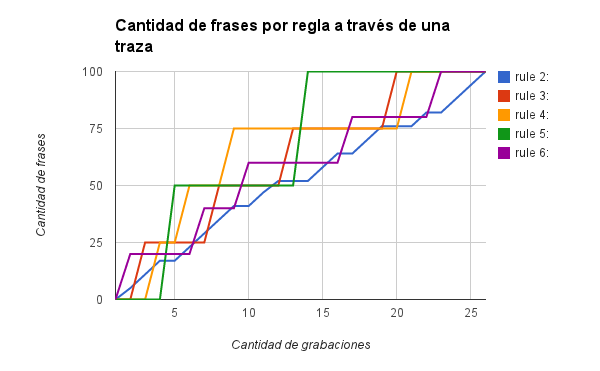
\includegraphics[width=0.9\textwidth]{cant_frases_traza_inf} }
    \caption{Cantidad de frases por traza}
    \label{figFracesTraza}
\end{figure}

En conclusión, se grabarán de a 5 frases. Teniendo en cuenta que las primeras serán frases conocídas y las últimas 2 corresponderán al esquema AMPER. 
